\chapter{Grundlæggende}

\section{Königsberg-Problemet}%
\label{sec:label}

Königsberg-problemet er ofte sagt til at være problemet der ``startede'' graf-teori. Beboerne af Königsberg i Preussen (i dag er dette \href{https://en.wikipedia.org/wiki/Kaliningrad}{Kaliningrad, Rusland}). Beboerne ville vide om det var muligt at gå over alle 7 broer blandt de to øer og land, og komme tilbage til hvor man startede.

\begin{figure}[ht]
  \centering
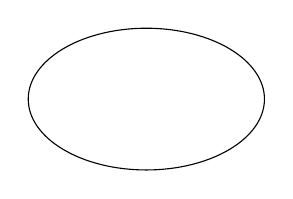
\begin{tikzpicture}
  \draw (0,0) ellipse (1.5 and 0.9);
\end{tikzpicture}
  \caption{\label{fig:konigsberg} Königsberg Broer}
\end{figure}




%%% Local Variables:
%%% mode: latex
%%% TeX-engine: xetex
%%% TeX-command-extra-options: "-shell-escape"
%%% TeX-master: "main"
%%% End:
